\chapter{Introduction to DUNE}
\label{ch:exec-overall}

%%%%%%%%%%%%%%%%%%%%%%%%%%%%%%%%%%%%%%%%%%%%%%%%%%%%%%%%%%%
\section{Overview}
\label{sec:exec-overall-1}

The Deep Underground Neutrino Experiment (DUNE) will be a world-class neutrino observatory and nucleon decay detector designed to answer fundamental questions about the nature of elementary particles and their role in the universe. The international DUNE experiment, hosted by the U.S. Department of Energy's \fnal{}, will consist of a far detector to be located about \SI{1.5}{km} underground at the Sanford Underground Research Facility (\surf) in South Dakota, USA, at a distance of  \SI{1300}{\km} from \fnal{}, and a near detector to be located on site at \fnal in Illinois. The far detector will be a very large, modular liquid argon time-projection chamber (\lartpc) with a \fdfiducialmass (\SI{40}{\giga\gram}) fiducial mass of liquid argon. The liquid-argon technology 
has the unique capability to reconstruct neutrino interactions with image-like precision and unprecedented resolution. 

The DUNE detectors will be exposed to the world's most intense neutrino beam originating at \fnal{}. A high-precision near detector, located \SI{575}{m} from the neutrino source on the \fnal site, will be used to characterize the intensity and energy spectrum of this wide-band beam. The ability to compare the energy spectrum of the neutrino beam between the near and far detectors
is crucial for discovering new phenomena in neutrino oscillations. The Long-Baseline Neutrino Facility (LBNF), also hosted by \fnal, provides the infrastructure for this complex system of detectors at the Illinois and South Dakota sites. LBNF is responsible for the neutrino beam, the deep-underground site, and the infrastructure for the DUNE detectors. 

\begin{dunefigure}[DUNE collaboration global map]{fig:map2}{The international DUNE
collaboration. Countries with DUNE membership are shown in orange.}
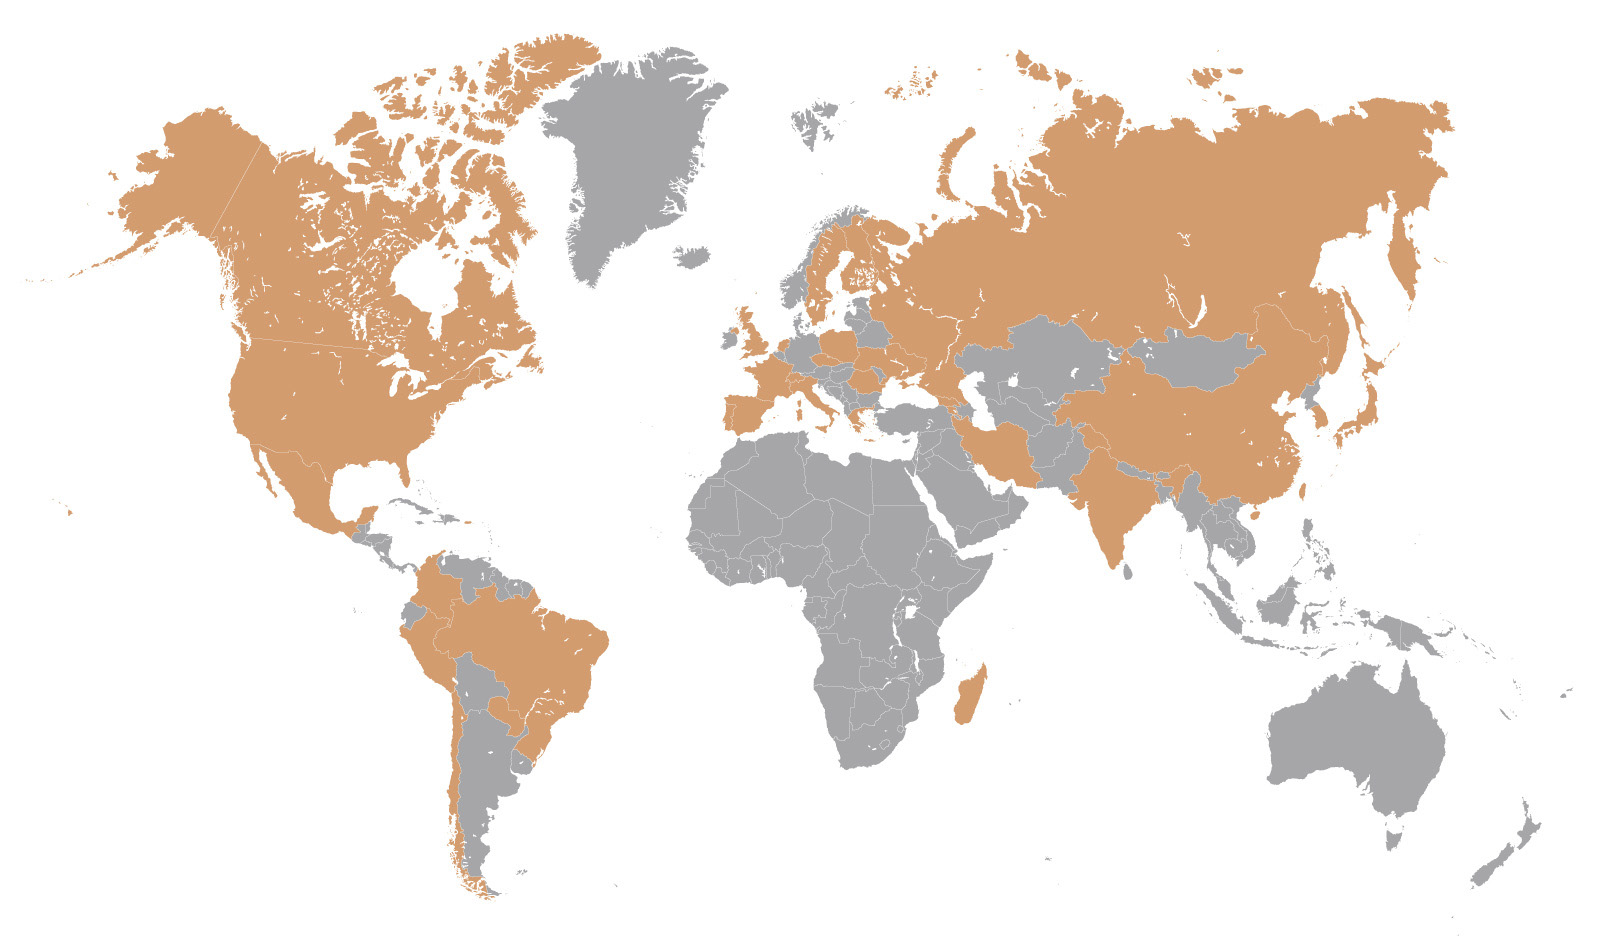
\includegraphics[width=0.9\textwidth]{dune-countries-july2019.jpg}  
\end{dunefigure} %updated by anne 7/15

The DUNE collaboration is a truly global organization including more than \num{1000} scientists and engineers from \num{31} countries (Figure~\ref{fig:map2}). It represents the culmination of several worldwide efforts that developed independent paths toward a next-generation long-baseline (LBL) neutrino experiment over the last decade. It was formed in April 2015, combining the strengths of the LBNE project in the USA and the LBNO project in Europe, adding many new international partners in the process. DUNE thus represents the convergence of a substantial fraction of the worldwide neutrino-physics community around the opportunity provided by the large investment planned by the U.S. Department of Energy (DOE) and \fnal to support a significant expansion of the underground infrastructure at \surf in South Dakota, and to create a megawatt neutrino-beam facility at \fnal by 2026. 
%{\it update} The Proton Improvement Plan-II (PIP-II) upgrade at \fnal~\cite{pip2-2013} will enable the accelerator to drive the new neutrino beamline with a \SI{80}{\GeV} primary proton beam at a beam power %from \SI{1.07}{\MW} 
%up to \pipiibeampower{}. A further planned upgrade 
of the accelerator complex will enable it to provide up to %\SI{2.4}{\MW} of beam power by 2030. 
%-- new version from Lia
The Proton Improvement Plan-II (PIP-II) accelerator upgrade at Fermilab~\cite{pip2-2013} will enable the world’s most intense beam of neutrinos to the international LBNF/DUNE experiment, as well as a broad physics research program. 
The PIP-II project will deliver between \SIrange{1.0}{1.2}{\MW} of proton beam power from the Main Injector in the energy range \SIrange{60}{120}{\GeV} at the start of DUNE, and provide a platform for extension of beam power to DUNE to multi-MW capability (>\SI{2}{\MW}). 
The CW-compatible, modern superconducting rf linac of PIP-II will increase the reliability of the Fermilab accelerator complex and provide flexibility through customized  beams tailored to specific scientific needs.  


The LBNF/DUNE strategy presented in this Technical Design Report (TDR) has been developed to meet the requirements set out in the report of the Particle Physics Project Prioritization Panel (P5 in 2014). It also takes into account the recommendations of the European Strategy for Particle  Physics (ESPP) adopted by the CERN Council in 2013, which classified the \dword{lbl} neutrino program as one of the four scientific objectives that require international infrastructure.
%which recommends development of
%a program to pave the way for a substantial European role in future long-%baseline experiments.

The P5 report~\cite{p5report} set the goal of reaching a sensitivity to \dword{cpv} of better than three standard deviations (\num{3}$\sigma$) over more than $75\%$ 
of the range of possible values of the unknown \dshort{cp}-violating phase \deltacp.
Based partly on this goal, they stated that ``the 
minimum requirements to proceed are the identified capability to reach an exposure 
of \num{120}~\ktMWyr{} by the 2035 time frame, the far detector situated underground 
with cavern space for expansion to at least \fdfiducialmass \lar fiducial volume, and \SI{1.2}{MW} 
beam power upgradeable to multi-megawatt power.
The experiment should have the demonstrated 
capability to search for \dwords{snb} and for proton decay, providing a significant 
improvement in discovery sensitivity over current searches for the proton lifetime.'' The strategy and design presented in this TDR meet these requirements.

This multi-volume document is the TDR for the DUNE Far Detector and covers the technology choices for the first three far detector modules. The type of LAr 
technology used for the fourth module is still to be decided. The TDR is intended to provide a clear statement of the physics goals of the DUNE collaboration, and to describe the detector designs that we believe will achieve these goals. The TDR includes dedicated volumes on the DUNE physics program, the DUNE far detectors, and the DUNE Technical Coordination organization. In addition to overviews of the other volumes, this executive summary volume also includes dedicated chapters on the near detector and computing, which will be the subject of future TDRs.

\section{Primary Science Goals}


The DUNE experiment will combine the world's most intense neutrino beam, a deep underground site, massive LAr detectors and a capable near detector to enable a broad science program addressing some of the most fundamental questions in particle physics. 
The primary science goals of DUNE, described in detail in Chapter~\ref{ch:phys-exec-summ}, are to: 
\begin{itemize}

\item Carry out a comprehensive program of neutrino oscillation measurements using \numu and \anumu beams from \fnal. This program includes measurements of the  \dword{cp} phase $\deltacp$, determination of the neutrino mass ordering (the sign of \dm{31}$ \equiv m_3^2-m_1^2$), measurement of the mixing angle $\theta_{23}$ and the determination of the octant in which this angle lies,
and sensitive tests of the three-neutrino paradigm. Paramount among these is the discovery of \dword{cp} violation in neutrino oscillations, which may give insight into the origin of the matter-antimatter asymmetry in the universe, one of the fundamental questions in particle physics and cosmology. 

\item Detect and measure the $\nu_\text{e}$ flux from a core-collapse supernova within our galaxy, should one occur during the lifetime of the DUNE experiment. Such a measurement would provide a wealth of unique information about the early stages of core-collapse, and could signal the birth of a black hole.
    
\item Search for proton decay in important decay modes and for other baryon number violating processes. The observation of baryon number violation would represent a ground-breaking discovery in physics, providing a key requirement for grand unification of the forces. 

\end{itemize}

The intense neutrino beam from LBNF, the massive DUNE \lartpc far detector, and the high-resolution
DUNE near detector will also provide a rich ancillary science program, beyond the primary goals of the experiment. The ancillary science program includes
\begin{itemize}
     \item other accelerator-based neutrino flavor transition measurements with sensitivity to beyond the standard model (BSM) physics, such as non-standard interactions (NSIs), Lorentz violation,  violation of the \dword{cpt}, the existence of sterile neutrinos, large extra dimensions, and heavy neutral leptons;
     \item measurements of tau neutrino appearance.
     \item measurements of neutrino oscillation phenomena using atmospheric neutrinos;
     \item a rich neutrino interaction physics program utilizing the DUNE near detector, including a wide-range of measurements of neutrino cross sections and studies of nuclear effects; %, including neutrino final-state interactions, measurements of the structure of nucleons, and  measurement of $\sin^2\theta_\text{W}$;
     \item  searches for dark matter.
\end{itemize} 
Further advancements in the \lartpc %far detector 
technology during the course of the DUNE far detector construction may open up the opportunity
to observe very low-energy phenomena such as solar neutrinos or even the diffuse supernova neutrino flux.


%%%%%%%%%%%%%%%%%%%%%%%%%%%%%%%%%%%%%%%%%%%%%%%%%%%%%%%%%%%%%%%
\section{The LBNF Facility} 

The organization and management of the Long-Baseline Neutrino
Facility (LBNF), hosted by Fermilab, is separate from the DUNE collaboration and is intended to enable the construction and operation of the DUNE detectors in South Dakota and Illinois.
The DUNE collaboration will construct a deep-underground neutrino observatory in South Dakota based on four independent liquid-argon TPC modules of 10 kt fiducial mass
and a high-precision, movable near detector at Fermilab comprising a liquid-argon TPC, a gas-argon TPC and a beam spectrometer. 
To enable this scientific program for the DUNE experiment,
LBNF will provide the facilities in Illinois and South Dakota.
These facilities are geographically separated into the near site facilities, to be constructed
at \fnal, and the far site facilities, located at \surf. Figure~\ref{fig:lbnf} shows
a schematic of the facilities at the two sites, and Figure~\ref{fig:caverns} shows a diagram of the cavern layout. 

\begin{dunefigure}[ 	
LBNF/DUNE project: beam from Illinois to South Dakota]{fig:lbnf}{ 	
LBNF/DUNE project: beam from Illinois to South Dakota.}
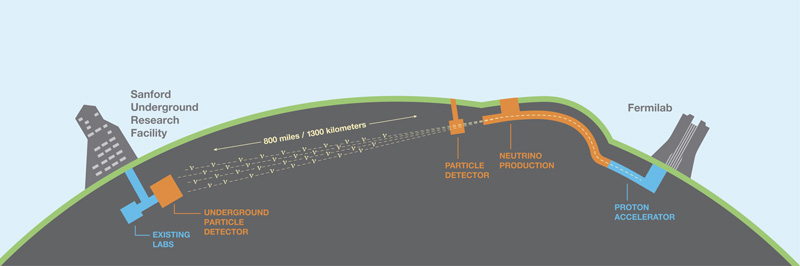
\includegraphics[width=0.9\textwidth]{lbnf_dune_graphic_miles_km-15-0031-01.jpg}
%\label{fig:mhexec}
\end{dunefigure}

Specifically, the Long-Baseline Neutrino Facility (LBNF) provides
\begin{itemize}
\item  the  technical and conventional facilities for a powerful neutrino beam utilizing the PIP-II upgrade of the \fnal accelerator 
complex, The PIP-II project will deliver between $1.0$--$1.2$~MW of proton beam power from the Main Injector in the energy range $60$--$120$~GeV at the start of DUNE, and provide a platform for extension of beam power to DUNE to multi-MW capability ($>2$~MW). 

\item  the civil construction, or \dword{cf}, for the near detector systems at \fnal; (see Figure~\ref{fig:beamline});

\item the excavation of three underground caverns at \surf. The north and south caverns will each house two cryostats with a
a minimum \nominalmodsize fiducial mass of liquid argon, while the central utility cavern will house cryogenics and data acquisition facilities for all four detector modules;

\item surface, shaft, and underground infrastructure to support 
the outfitting of the caverns with four free-standing, steel-supported cryostats 
and the required cryogenics systems to enable a rapid deployment of the first two \nominalmodsize far detector modules. 
The intention is to install the third and fourth cryostats as rapidly as funding will 
allow.
\end{itemize}

\begin{dunefigure}[ 	
Underground caverns for DUNE in South Dakota]{fig:caverns}{Underground caverns for DUNE far detector and cryogenics systems at \dword{surf}, in South Dakota. The drawing shows the first two far detector modules in place.}
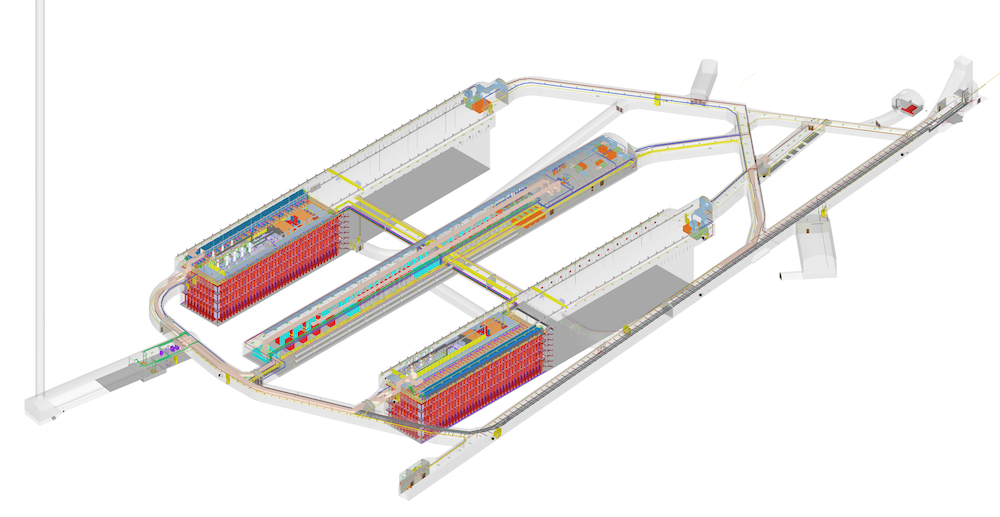
\includegraphics[width=0.99\textwidth]{caverns_full_assembly}
\end{dunefigure}

\begin{dunefigure}[Neutrino beamline and DUNE near detector hall in Illinois
]{fig:beamline}{Neutrino beamline and DUNE near detector hall at Fermilab, in Illinois}
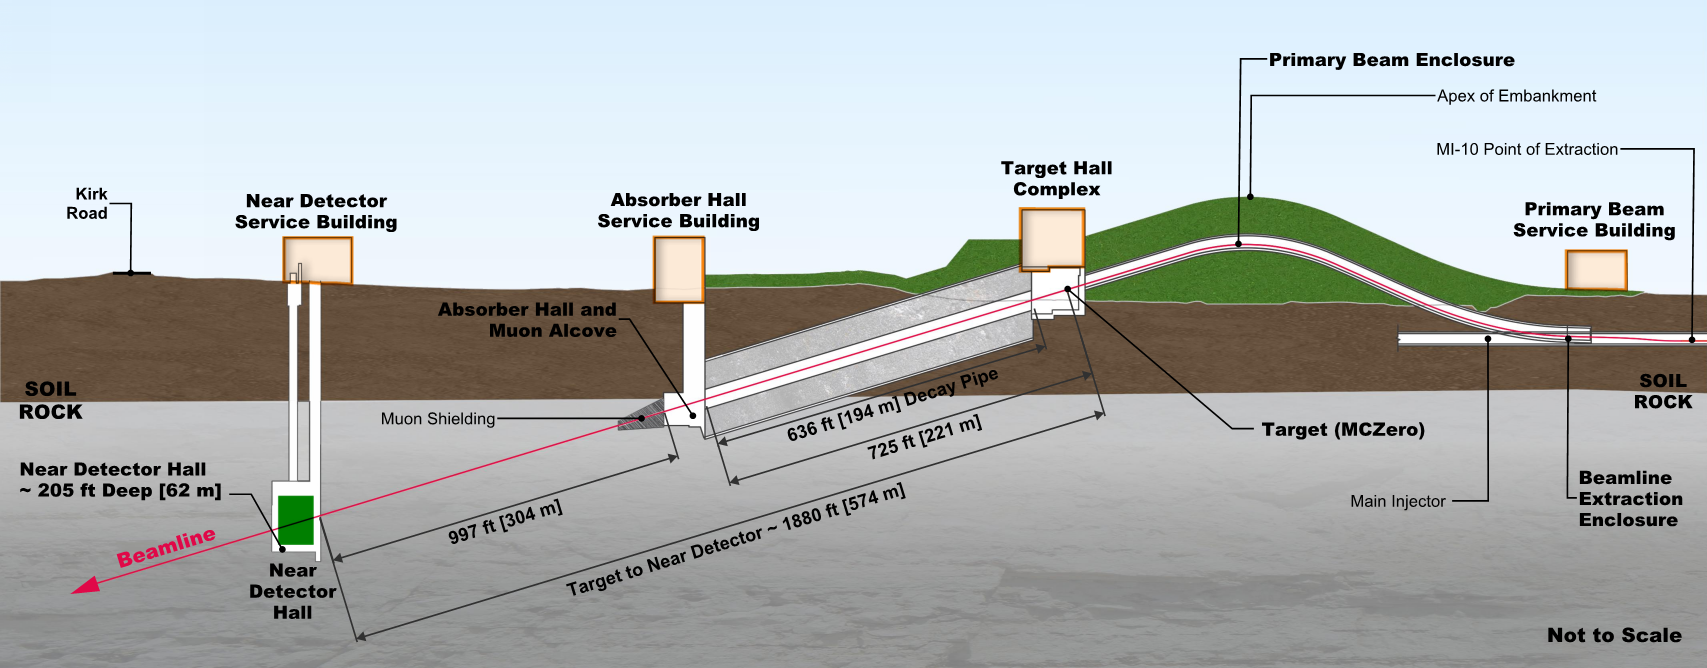
\includegraphics[width=0.95\textwidth]{beamline-sideview.jpg}
\end{dunefigure}


%The success of the DUNE project depends on the successful realization of the LBNF facilities.
%This \dword{tp} focuses on the DUNE physics program that is enabled by
%the first three \dword{fd} modules, which are expected to be based on the \dword{sp} and \dword{dp} \lar technologies.

\section{The DUNE Experiment}

The DUNE experiment includes a precision near detector at the edge of the \fnal site, in Batavia, Illinois, and a very large, modular far detector about \SI{1.5}{km} underground at \surf in Lead, South Dakota, \SI{1300}{km} (\SI{800}{miles}) from \fnal. The DUNE far detector is the focus of this \dword{tdr}. 

% ecb: Do ProtoDUNEs show up here or in a separate section? Somewhere, we need to state what specific performance measures we are counting on having from ProtoDUNE before the TDR.

\subsection{Far Detector}
\label{ch:dune-det-tech-ov-fd}

%The DUNE \dword{fd} will consist of four similar \lartpc{}s, each with fiducial mass of at least \nominalmodsize, installed about \SI{1.5}{km} underground. Each detector will be installed in a cryostat with internal dimensions
%\cryostatwdth (W) $\times$ \cryostatht (H) $\times$ \cryostatlen (L), and will contain a total \lar{} mass of about \larmass{}.
%The \lartpc technology provides
%excellent tracking and calorimetry performance, making it an ideal
%choice for the DUNE far detectors. The four identically sized cryostats give flexibility for staging and evolution of the \lartpc technology.

%DUNE is planning for and prototyping two \lartpc technologies:
%\begin{itemize}
%\item Single-phase (SP): This technology was pioneered by the ICARUS project, and after several decades of worldwide R\&D, is now a mature technology. It is the technology used for \fnal{}'s currently operating \microboone, and the planned SBND. In the \single technology, ionization charges are drifted horizontally in \lar and read out on wires in the liquid. The maximum drift length in the DUNE \dword{spmod} is \spmaxdrift and the nominal drift field is \spmaxfield, corresponding to a cathode high voltage of \sptargetdriftvoltpos. There is no signal amplification in the liquid, so readout with good signal-to-noise requires very low-noise electronics.

%\item Dual-phase (DP): This technology was pioneered at large scale by the \dword{wa105} collaboration. It is less established than the \single technology but offers a number of potential advantages and challenges. Here, ionization charges are drifted vertically in \lar and transferred into the gas above the liquid. The signal charges are then amplified in the gas phase using large electron multipliers (LEMs). This gain reduces the requirements on the electronics, and makes it possible for the \dword{dpmod} to have a longer drift, which requires a correspondingly higher voltage.
%The maximum drift length in the \dword{dpmod} is \dpmaxdrift and the nominal drift field is \dpnominaldriftfield, corresponding to a cathode high voltage of \dptargetdriftvoltpos. 

%\end{itemize}

%The plans for the single and dual-phase TPCs are described briefly in the following sections, and in detail in Volumes 3 and 4 of this \dword{tdr}.

%The DUNE collaboration is committed to deploying both technologies. 
%For planning purposes, DUNE assumes the first \dword{detmodule} to be
%\single and the second to be \dual.
%The actual sequence of \dword{detmodule} installation will depend on results from the prototype detectors, described below, and on available resources.

%--- add sections from Anne's document:
%
%\section{The Far Detector}


The \fdfiducialmass \dword{dune} \dword{fd} will consist of four \dword{lartpc} \dwords{detmodule}, each with fiducial mass of at least \nominalmodsize, installed approximately \SI{1.5}{km} underground. The \dword{lartpc} technology provides
excellent tracking and calorimetry performance, making it an ideal
choice for the DUNE \dword{fd}. Each of the \dwords{lartpc} fits inside a cryostat of internal dimensions
\cryostatwdth (W) $\times$ \cryostatht (H) $\times$ \cryostatlen~(L) that contains a total \lar{} mass of about \larmass{}.
 The four identically sized modules provide flexibility for staging construction and for evolution of \dword{lartpc} technology.

DUNE is planning for and is prototyping two \dword{lartpc} technologies:
\begin{itemize}
\item \Dword{sp}: In the \dword{sp} technology, ionization charges are drifted horizontally in \dword{lar} and read out on wires in the liquid.  The maximum drift length in the first DUNE \dword{spmod} is \spmaxdrift and the nominal drift field is \spmaxfield, corresponding to a cathode \dword{hv} of \sptargetdriftvoltpos. This design requires very low-noise electronics to achieve readout with good signal over noise (\dword{s/n}) since no signal amplification takes place in the liquid. This technology was pioneered by the \dword{icarus} project, and after several decades of worldwide R\&D, is now a mature technology. It is the technology used for \dword{fnal}'s currently operating \dword{microboone} detector, and the \dword{sbnd} detector which is currently under construction. 

\item \Dword{dp}: This technology was pioneered at a large scale by the \dword{wa105} collaboration at CERN. It is less established than the \dword{sp} technology but offers a number of potential advantages and challenges. Here, ionization charges drift vertically in \dword{lar} and are transferred into a layer of gas above the liquid. Devices called \dwords{lem} amplify the signal charges  in the gas phase. The gain achieved in the gas reduces the stringent requirements on the electronics, and increases the possible drift length, which, in turn, requires a correspondingly higher voltage. The nominal drift field is \dpnominaldriftfield as for the SP detector, but in this case corresponds to a cathode \dword{hv} of \dptargetdriftvoltpos.
The maximum drift length in the \dword{dpmod} is \dpmaxdrift{}.  
\end{itemize}
%from Justin's SP exec summ
In both technologies, the drift volumes are surrounded by a \dword{fc} that defines the volume(s) and ensures uniformity of the \efield to 1\% within the volume.

Liquid argon is an excellent scintillator at a wavelength of \SI{126.8}{\nano\meter}. This fast scintillation light, once shifted into the visible spectrum, is collected by \dwords{pd} in both designs. The \dwords{pd} provide a time $t_{0}$ for every event, indicating when the ionization electrons begin to drift. Comparison of the time at which the ionization signal reaches the anode relative to the time $t_{0}$ allows reconstruction of the event topology in the drift coordinate; the precision of the measured $t_{0}$, therefore, directly corresponds to the precision of the spacial reconstruction in this direction. 

Two key factors affect the performance of the \dword{dune} \dwords{lartpc}.  First, the \dword{lar} purity must be high enough to achieve minimum charge attenuation over the longest drift lengths in a given \dword{detmodule}.  Thus, the levels of electro-negative contaminants (e.g., oxygen and water) must be maintained at ppt levels.  The \dword{sp} and \dword{dp} designs have slightly different purity requirements (expressed in minimum electron lifetimes of \SI{3}{ms} versus \SI{5}{ms}) due to the different drift lengths.

Second, the electronic readout of the \dword{lartpc} requires very low noise levels to allow the signal from the drifting electrons to be clearly discernible over the baseline of the electronics.  This requires use of low-noise cryogenic electronics. 

The plans for the single and dual-phase TPCs are described briefly in the following sections, and in detail in Volumes 3 and 4 of this \dword{tdr}.
The DUNE collaboration is committed to deploying both technologies. 
For planning purposes, we assume that the first \dword{detmodule} will be
\single and the second will be \dual.
The actual sequence of \dword{detmodule} installation will depend on results from the prototype detectors, described below, and on available resources.

The full DUNE far detector requires four modules. For the \dword{tdr}, we will describe plans for the first three of these modules: two \dwords{spmod}, one of which will be the first module installed, and one \dword{dpmod}. Resources for the fourth \dword{detmodule}, which may employ a more advanced design, remain to be identified. 

%%%%%%%%%%%%%%%%%%%%%%%%%%%%%%%%%%%%%%%%
\subsubsection{Single-Phase Technology}
\label{sec:fdsp-exec-splar}

Figure~\ref{fig:LArTPC1} shows the general operating principle of the \dword{sp} \dword{lartpc}, as has been previously demonstrated by  \dword{icarus}~\cite{Icarus-T600}, \dword{microboone}~\cite{microboone}, \dword{argoneut}~\cite{Anderson:2012vc}, \dword{lariat}~\cite{Cavanna:2014iqa}, and \dword{protodune}~\cite{Abi:2017aow}. Figure~\ref{fig:DUNESchematic1} shows the configuration of a \dword{dune} \dword{spmod}. Each of the four drift volumes of \dword{lar} is subjected to a strong electric field of \spmaxfield. Charged particles passing through the \dword{tpc} ionize the argon, and the ionization electrons drift in the electric field to the anode planes. 

\begin{dunefigure}[The SP LArTPC operating principle]{fig:LArTPC1}
{The general operating principle of the \dword{sp} \dword{lartpc}.}
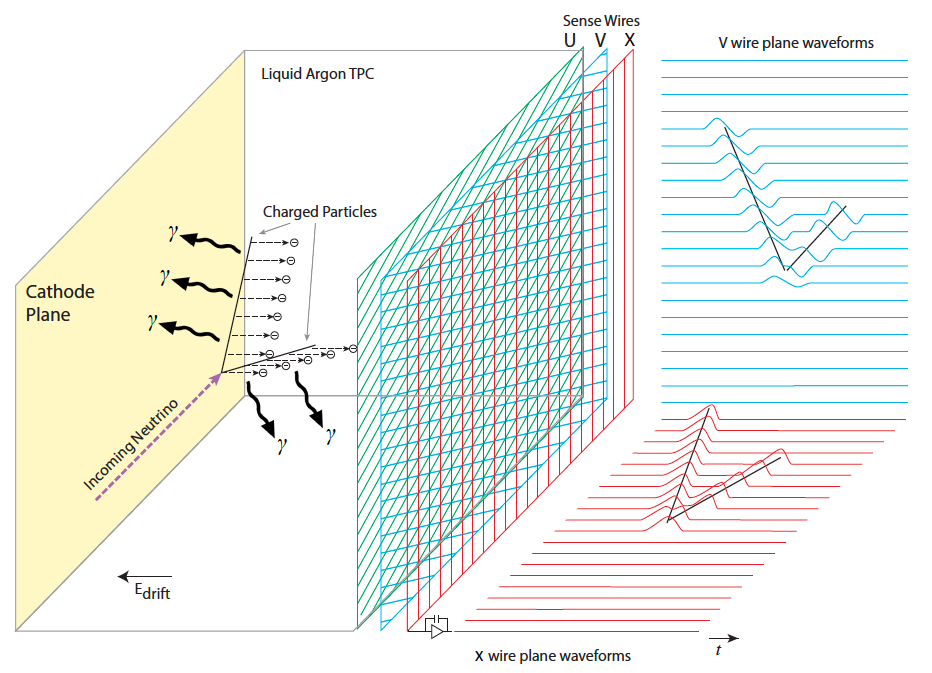
\includegraphics[width=0.75\textwidth]{TheBoPicture.png} 
\end{dunefigure}

A \dword{spmod} is instrumented with three module-length anode planes constructed from \SI{6}{m} high by \SI{2.3}{m} wide \dwords{apa}, stacked two APAs high and 25 wide, for 50 \dwords{apa} per plane, or 150 total. Each \dword{apa} consists of three layers of active wires forming a grid. The relative voltage between the layers is chosen to ensure the transparency of the first two layers ($U$ and $V$) to the drifting electrons. These layers produce bipolar induction signals as the electrons pass through them. The final layer ($X$) collects the drifting electrons, resulting in a uni-polar signal. The pattern of ionization collected on the grid of anode wires provides the reconstruction in the remaining two coordinates perpendicular to the drift direction.

\begin{dunefigure}[A \nominalmodsize DUNE far detector SP module.]{fig:DUNESchematic1}
{Schematic of a \nominalmodsize \dword{dune} \dword{fd} \dword{spmod}, showing the alternating anode (A) and cathode (C) planes that divide the \dword{lartpc} into four separate drift volumes. The red arrows point to one top and one bottom \dword{fc} module and to the rear \dword{ewfc}.}
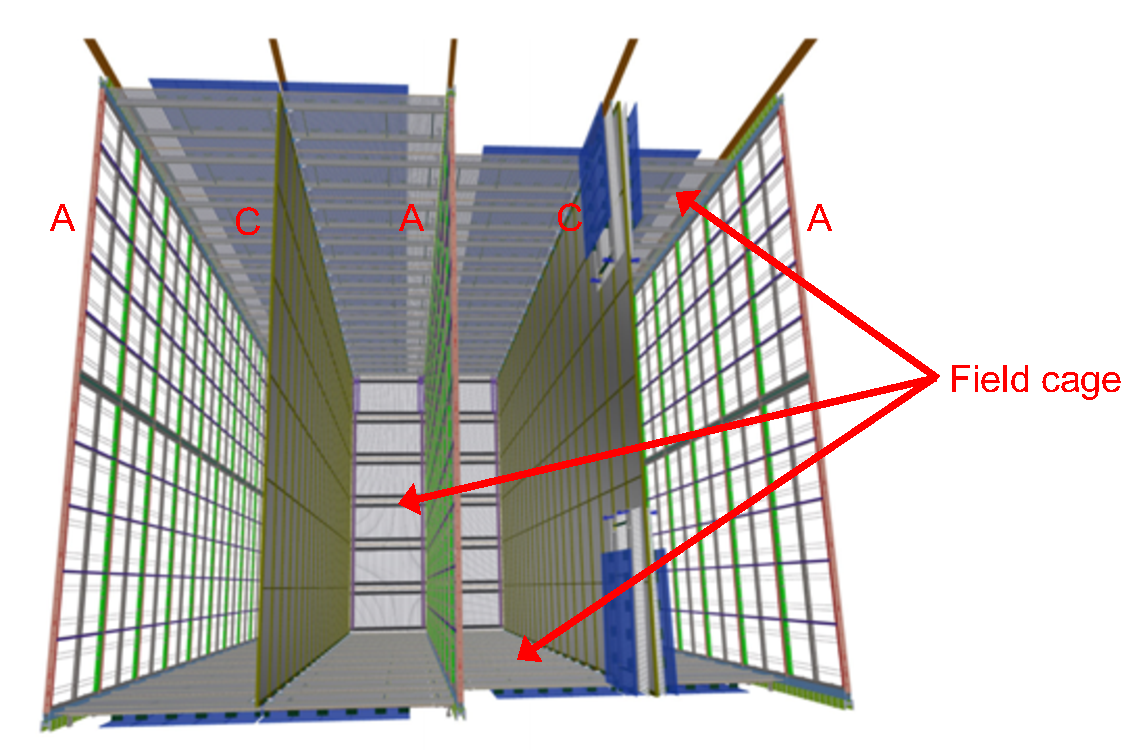
\includegraphics[width=0.65\textwidth]{DUNESchematic.pdf}
\end{dunefigure}

Novel \Dword{pd} collector modules (called ARAPUCAs) using \dwords{sipm} are placed in the inactive space between the innermost wire planes of the \dword{apa}s, installed through slots in a pre-wound \dword{apa} frame. 
There are ten \dword{pd} modules per \dword{apa} for a total of \num{1500} per \dword{spmod}.  Of these, \num{500} are mounted in central \dword{apa} frames and must collect light from both directions, 
and \num{1000} are mounted in frames  near the vessel walls and collect light from only one direction. 

\FloatBarrier
%%%%%%%%%%%%%%%%%%%%%%%%%%%%%%%%%%%%%%%%
\subsubsection{Dual-Phase Technology}
\label{sec:fddp-exec-splar}

The \dword{dp} operating principle, illustrated in Figure~\ref{fig:figure-label-DPprinciple} is very similar to that of the \dword{sp} design.  Charged particles that traverse the active volume of the \dword{lartpc} ionize the medium while also producing scintillation light.  The ionization electrons drift along an \efield towards a segmented anode where they deposit their charge, and where  \dwords{pd} pick up the scintillation light. 

The key differentiating concept of the \dword{dp} design is the amplification of the ionization signal in an avalanche process that takes place in a layer of argon gas above the \dword{lar}.  
In this design, shown in Figure~\ref{fig:DPdet1}, electrons drift upward toward an extraction grid just below the liquid-vapor interface. 
After reaching the grid, an \efield stronger than the \dpnominaldriftfield{} drift field extracts the electrons from the liquid up into the gas phase. Once in the gas, electrons encounter micro-pattern gas detectors, called \dwords{lem}, with high-field regions. The \dwords{lem} amplify the electrons in avalanches that occur in these high-field regions. The amplified charge is then collected and recorded on a \twod anode
consisting of two sets of %\SI{3.125}{mm}-pitch 
gold-plated copper strips that provide the $x$ and $y$ coordinates (and thus two views) of an event. 

 The extraction grid, \dword{lem}, and anode are assembled into three-layered sandwiches with precisely defined inter-stage distances and inter-alignment,  which are then connected together horizontally into \num{9}~m$^2$ modular detection units. These detection units are called \dwords{crp}.

The precision tracking and calorimetry offered by the \dword{dp} technology provides excellent capabilities for identifying interactions of interest while mitigating sources of background.  Whereas the \dword{sp} design has multiple drift volumes, the \dword{dpmod} design allows a single, fully homogeneous \dword{lar} volume with a much longer drift length.

An array of \dwords{pmt} coated with a wavelength-shifting material is located below the cathode. The \dwords{pmt} record  the time and pulse characteristics of the incident light.


\begin{dunefigure}[The DP LArTPC operating principle]{fig:figure-label-DPprinciple}{The general operating principle of the \dword{dp} \dword{lartpc}.}
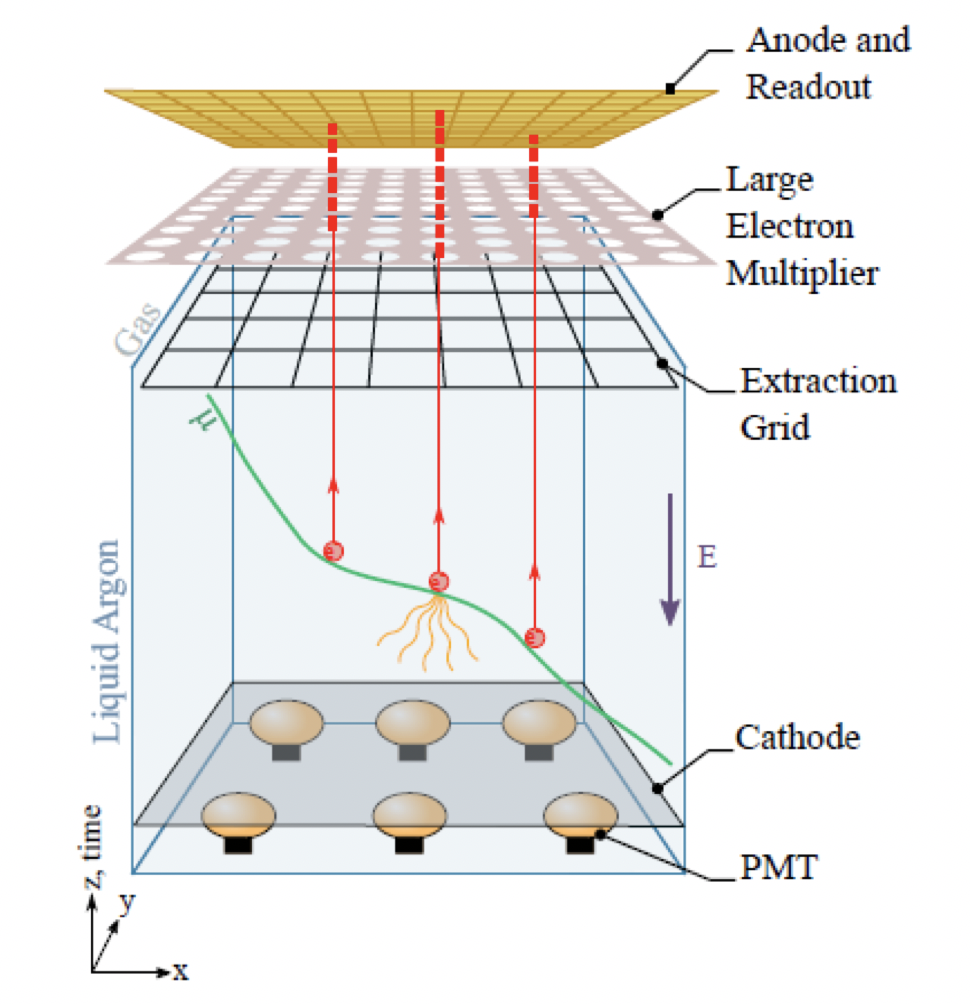
\includegraphics[width=0.5\textwidth]{dualphase-principle}
\end{dunefigure}

\begin{dunefigure}[A \nominalmodsize DUNE Far Detector DP module.]{fig:DPdet1}
  {Schematic of a \nominalmodsize DUNE \dword{fd} \dword{dp} \dword{detmodule} with cathode, \dwords{pmt}, \dword{fc}, and anode plane with \dwords{sftchimney}.}
  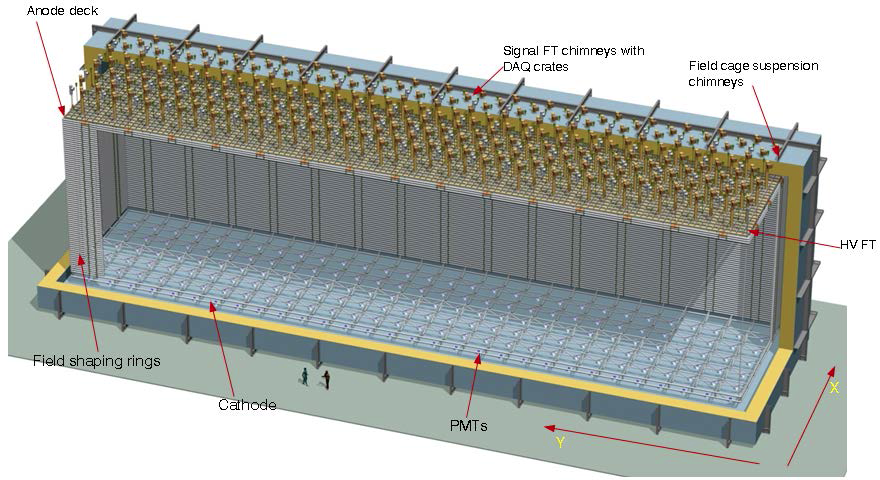
\includegraphics[width=0.9\textwidth]{DUNE-CDR-detectors-volume-optim.png}
\end{dunefigure}
\FloatBarrier
%%%%%%%%%%%%%%%%%%%%%%%

\subsubsection{ProtoDUNEs: Far Detector Protptypes}

The DUNE collaboration has constructed 
two large prototype detectors (\dwords{protodune}), one employing \single readout (\dword{pdsp}) and the other \dual readout (\dword{pddp}). Each is approximately one-twentieth of a DUNE \dword{detmodule}, but uses components identical in size to those of the full-scale module. \dword{pdsp} has the same \spmaxdrift maximum drift length as the full \dword{spmod}. \dword{pddp} has a \SI{6}{m} maximum drift length, half of that planned for the \dword{dpmod}. 

\begin{dunefigure}[ProtoDUNE-SP and ProtoDUNE-DP cryostats in the CERN Neutrino Platform in CERN's North Area.]
{fig:protodunes_northarea}
{ProtoDUNE-SP and ProtoDUNE-DP cryostats in the CERN Neutrino Platform in CERN's North Area.}
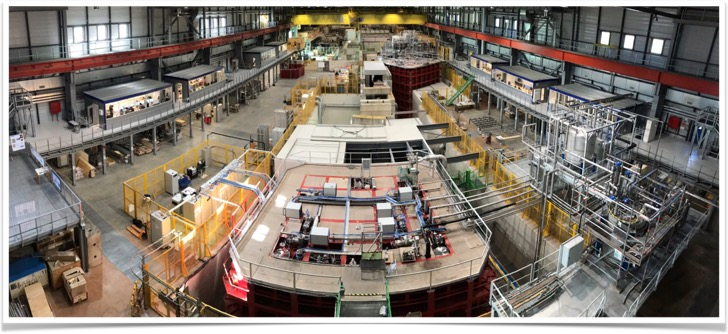
\includegraphics[width=0.9\linewidth]{neutrinoplatform.jpg}
\end{dunefigure}

\begin{dunefigure}[Interior views of ProtoDUNE-SP (one of two drift volumes) (left) and ProtoDUNE-DP (right)]
{fig:protodunes_interior}
{Interior views of ProtoDUNE-SP (left) and ProtoDUNE-DP (right). For ProtoDUNE-SP, one of two identical drift volumes is shown.}
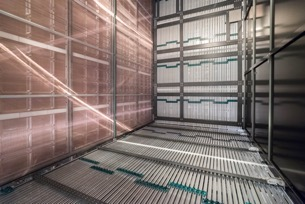
\includegraphics[width=0.46\linewidth]{graphics/ProtoDUNE-sp-interior.jpg}\hspace{0.05\linewidth}
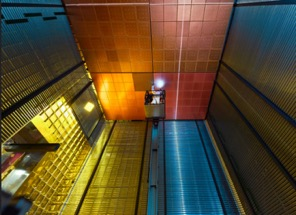
\includegraphics[width=0.44\linewidth]{graphics/protodune-dp-interior.jpg}
\end{dunefigure}

These large-scale prototypes will allow us to validate key aspects of the TPC designs, test engineering procedures, and collect valuable calibration data using a hadron test beam. The following list includes the key goals of the \dword{protodune} program:
\begin{enumerate}
\item Production of components:
\begin{itemize}
\item stress testing of the production and quality
assurance processes of detector components,
\item mitigation of the associated risks for the far detector.
\end{itemize}
\item Validate installation procedures:
\begin{itemize}
\item test of the interfaces between the detector elements,
\item mitigation of the associated risks for the far detector.
\end{itemize}
\item Detector operation with cosmic rays:
\begin{itemize}
\item validation of the detector designs and
performance.
\end{itemize}
\item Collection of test beam data:
\begin{itemize}
\item measurements of essential physics response of the detector.
\end{itemize}
\end{enumerate}


% -- (ed) I put DP sentence first to get it out of the way before the long SP discussion, but it may be too awkward this way.
 The construction of the ProtoDUNE-DP detector was completed in June of 2019, and the detector is expected to begin collecting cosmic-ray data in August 2019. The construction phase of \dword{pdsp} finished in July 2018, and the detector was filled with liquid argon in August 2018. The detector collected hadron beam data and cosmic rays during the fall of 2018, and continues to collect cosmic-ray data.

The data taken with the \dword{pdsp} detector demonstrates the excellent performance of the detector and has already provided valuable information on the design, calibration, and simulation of the DUNE far detector. In total, $99.7\%$ of the 15360 TPC electronics channels are responsive in the liquid argon. The equivalent noise charge (ENC) amounts to $\approx 550$ $e^{-}$ on the collection wires and $\approx 650$ $e^{-}$ on the induction wires. An average signal to noise ratio (S/N) of 38 for the collection plane is measured using cosmic-ray muons, while for the two induction planes, S/N$=14$ (U) and 17 (V), exceeding the requirement of a ratio $9:1$ for the DUNE far detector. 

\begin{dunefigure}[Calibrated $dE/dx$ vs residual range measured by TPC for 1 GeV/c stopping protons (left) and response of ARAPUCA photon-detector module in APA3 as a function of incident electron kinetic energy (right).]
{fig:pdtpcpd}
{Calibrated $dE/dx$ vs residual range measured by TPC for 1 GeV/c stopping protons (left) and response of ARAPUCA photon-detector module in APA3 as a function of incident electron kinetic energy (right).} 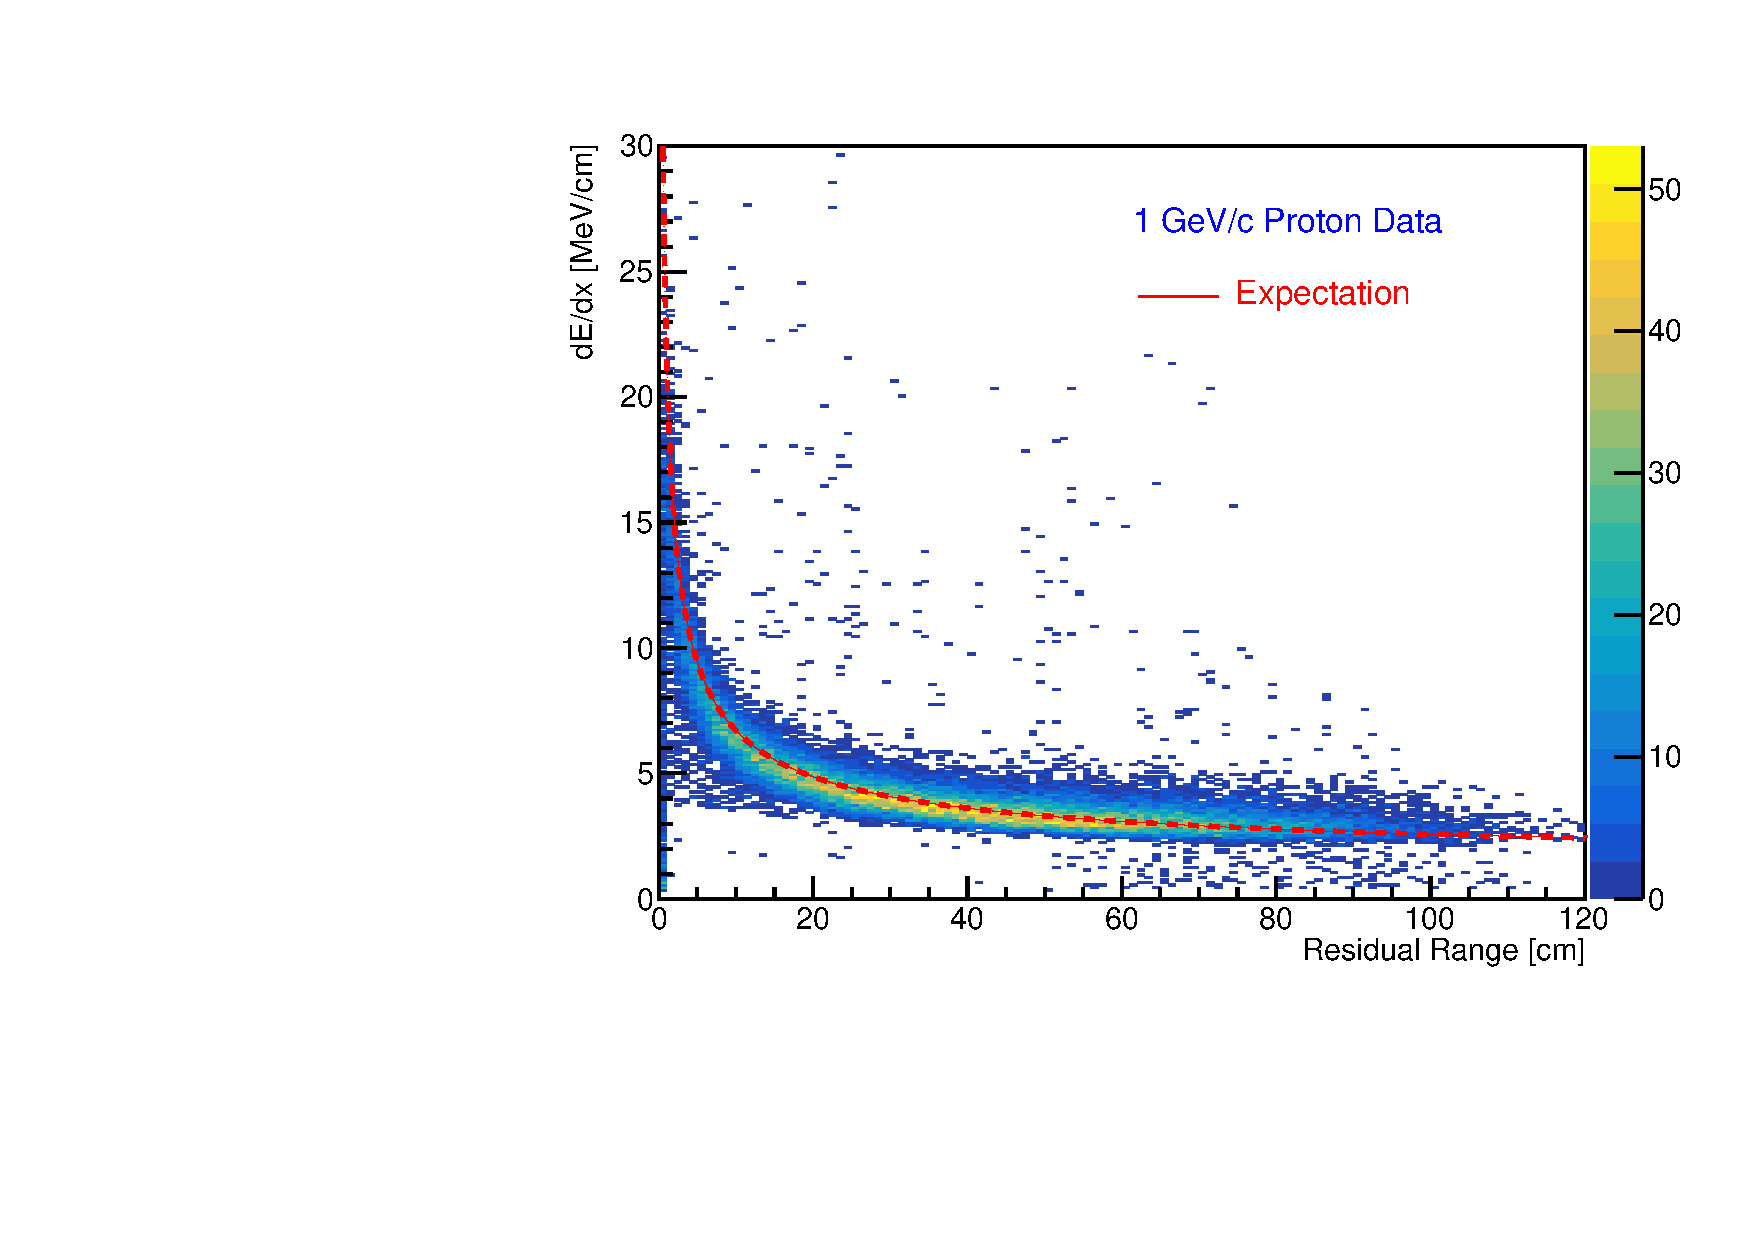
\includegraphics[width=0.47\linewidth]{graphics/dedx_rr_data_v5.pdf}
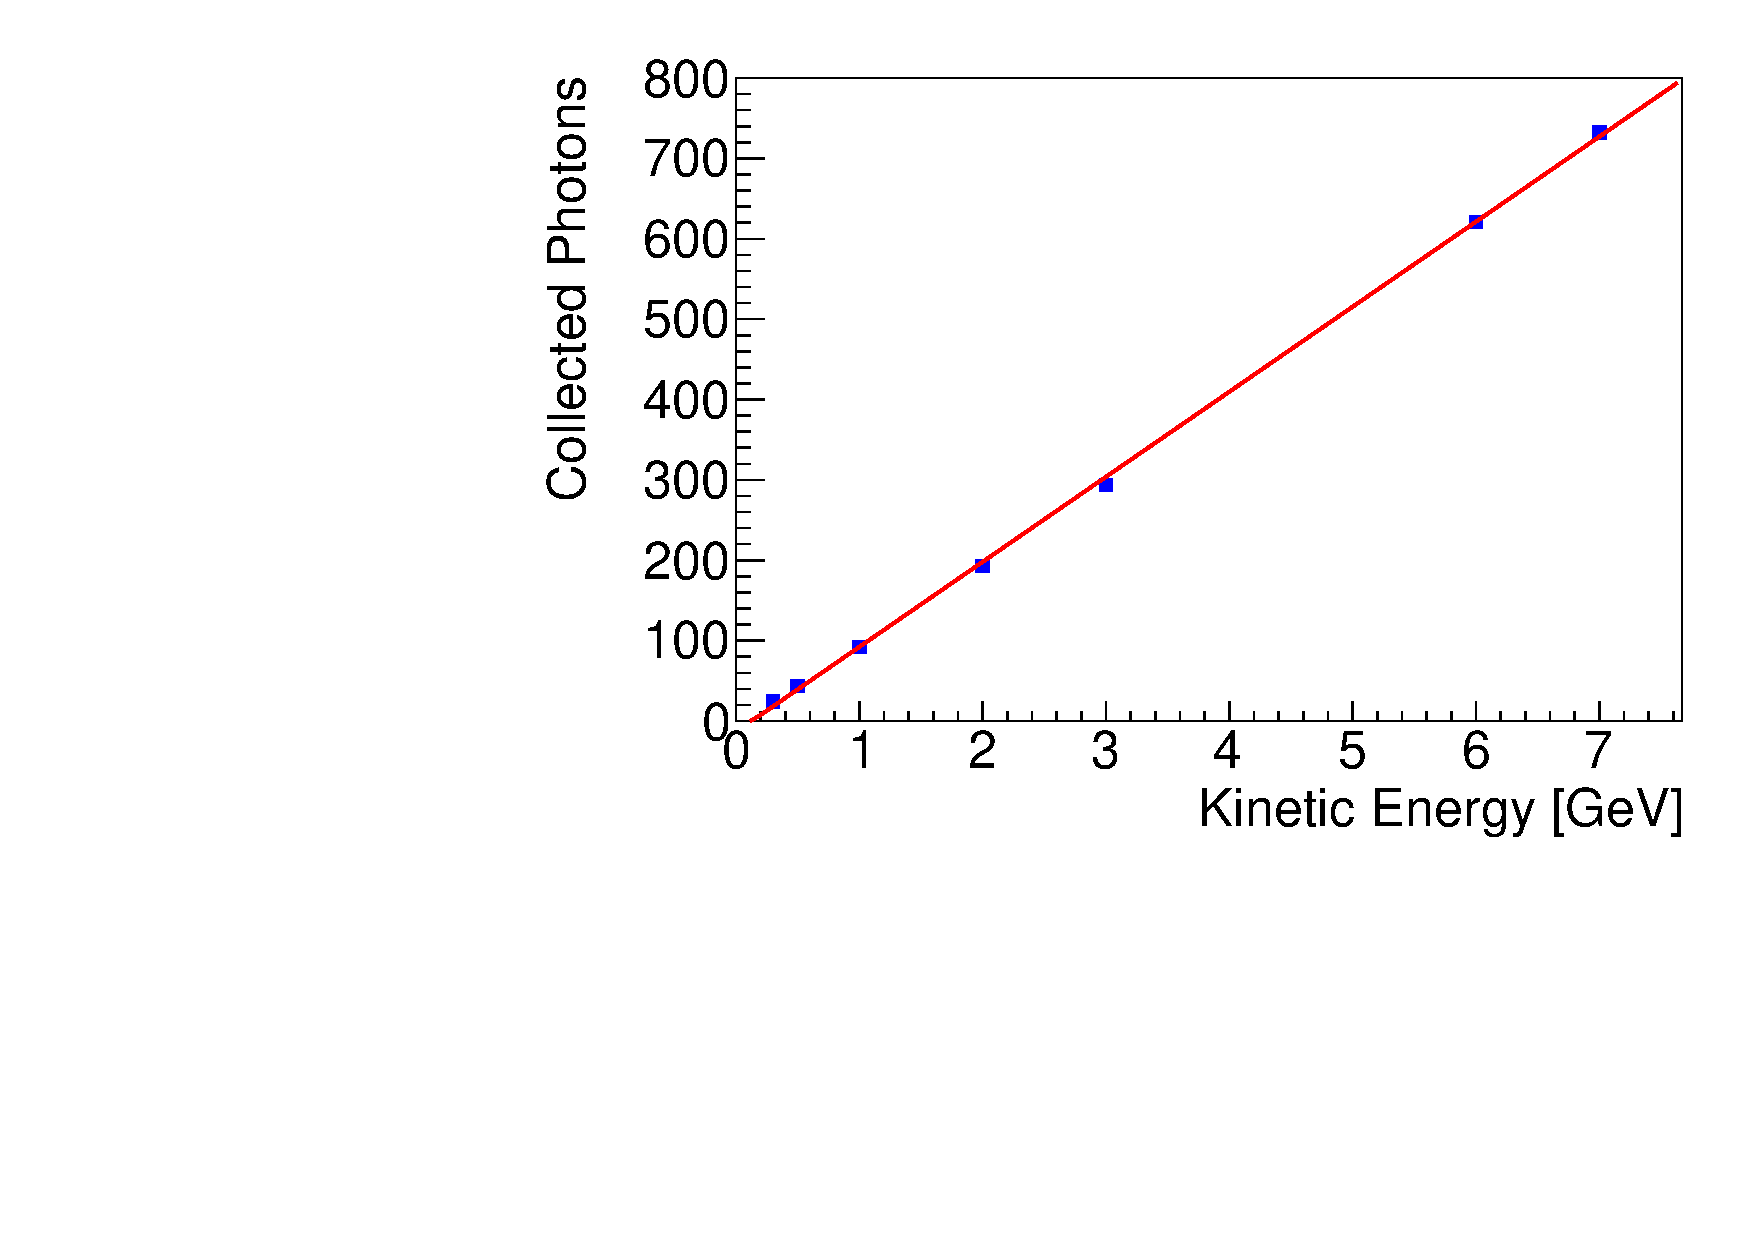
\includegraphics[width=0.5\linewidth]{pdsarapucabeamresponse.pdf}
\end{dunefigure}

As the detector is located on the surface, \dword{pdsp} sees an excess of ions accumulate in the drift volume that distorts the electric field and the reconstructed particle trajectories, which is known as the space charge effect (SCE). A calibration procedure removes the detector non-uniformity, which is dominated by the SCE. We then convert the charge deposited along the track to the energy loss ($dE/dx$) using stopping cosmic-ray muons. The calibration constants that have been derived with this method are applied to the energy deposits measured for the beam particles, including muons, pions, protons, and positrons.
The resulting $dE/dx$ distributions agree well with expectations.  Figure~\ref{fig:pdtpcpd}(left) shows the calibrated $dE/dx$ values as a function of the track residual range for protons in the 1 GeV/$c$ beam, in good agreement with expectations. 

The \dword{pdsp} beam run provides a unique set of high quality data for detector performance characterization, physics studies, and calibration. The data will also
allow us to perform hadron-argon cross-section measurements, which are relevant for future DUNE neutrino oscillation analyses.
Data collected during the beam run are also utilized for characterization of the Photon Detector System's (PDS) response to light signals. Other useful data sets include
beam data with triggers determined by the beam instrumentation, cosmic-ray data  from random triggers or from those in coincidence with the Cosmic Ray Tagger (CRT) modules, as well as calibration data, with triggers enabling programmed light pulses. 
The single avalanche response and gain for each of the 256 readout channels of the PDS have been determined from calibration data.
The initial analysis results illustrate a very good performance and stability of the photon system.

Figure~\ref{fig:pdtpcpd}(right) shows the response of an ARAPUCA photon-detector module as a function of incident electron kinetic energy
The observed number of photons has not been corrected for geometry and detection efficiency. The analysis serves to demonstrate the achieved energy linearity for beam electrons contained in the detector.  
In addition to understanding the PDS response and calibration, \dword{pdsp} demonstrated the excellent correlation between TPC timing and the PDS timing. The later will lead to further optimized physics reach of DUNE. 


\subsection{Near Detector}
\label{sec:nd-verview}

The \dword{dune} \dword{nd} is crucial for the success of the DUNE physics program. It is used to perform a precise measurement of the neutrino beam flux and flavor composition. The comparison of the measured neutrino energy spectra at the near and far site allows us to disentangle the different energy-dependent effects that modulate the beam spectrum and to reduce the systematic uncertainties to the level required for discovering CP violation. In addition, it will measure neutrino-argon interactions with high precision using both gaseous and liquid argon, which will further reduce the systematic uncertainties due to the modelling of these interactions.

\begin{dunefigure}[DUNE Near Detector]
{fig:neardetectors}
{DUNE Near Detector. The beam enters from the right and encounters
the \dword{lartpc}, the \dword{mpd}, and the on-axis beam monitor with the 3DST.}
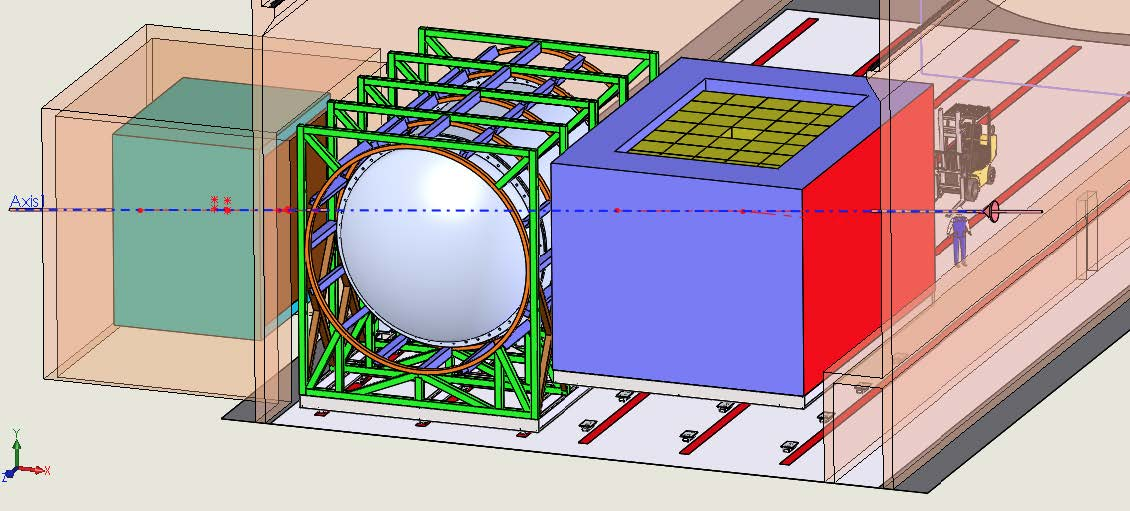
\includegraphics[width=0.9\textwidth]{ND_Detectors.jpg}
\end{dunefigure}


The \dword{nd} hall will be located \SI{575}{m} downstream from the target, and will include three primary detector components, shown in Fig.~\ref{fig:neardetectors}  and listed in Table~\ref{tab:NDsumm}. Two of them will be able to move off beam axis, providing access to different neutrino energy spectra. The movement off axis, called \dword{duneprism}, provides a crucial extra degree of freedom for the ND measurement, and is therefore an integral part of the DUNE Near Detector concept. 

The three detector components -- a \dword{lartpc} called \dword{arcube}, an \dword{hpgtpc} within a magnet surrounded by an \dword{ecal} (together called Multipurpose Detector or \dword{mpd}), and an on-axis beam monitor containing a \dword{3dst} surrounded by the KLOE magnet -- serve important individual and overlapping functions with regard to the mission of the \dword{nd}. 
The \dword{dune} \dword{nd} is shown schematically in the \dword{dune} \dword{nd} hall in Figure~\ref{fig:NDHallconfigs}.  Table~\ref{tab:NDsumm} provides a high-level overview of the three components of the \dword{dune} \dword{nd} along with the off-axis capability.  

\begin{dunetable}[Components of the DUNE ND]
{p{.22\textwidth}p{.22\textwidth}p{.22\textwidth}p{.22\textwidth}}
{tab:NDsumm}{This table gives a high-level breakdown of the three major detector components and the capability of movement for the DUNE ND along with function and primary physics goals.}
Component & Essential Characteristics & Primary function & Select physics aims \\ \toprowrule
LArTPC (ArgonCube) & Mass  & Experimental control for the Far Detector & $\numu$($\overline{\nu}_{\mu}$) CC \\
          & Target nucleus Ar &  Measure unoscillated $E_\nu$ spectra   & $\nu$-e$^{-}$ scattering   \\
          &  Technology FD-like    &  Flux determination  &  $\nue +$$\overline{\nu}_{e}$ CC  \\
          &  &  &  Interaction model \\ \colhline
Multipurpose detector (MPD) & Magnetic field & Experimental control for the LArTPCs & $\numu$($\overline{\nu}_{\mu}$) CC \\
  &  Target nucleus Ar & Momentum analyze liquid Ar $\mu$ & $\nue$ CC, $\overline{\nu}_{e}$ \\
  & Low density & Measure exclusive final states with low momentum threshold & Interaction model \\  \colhline
DUNE-PRISM (capability) & LArTPC$+$MPD move off-axis & Change flux spectrum &  Deconvolve xsec*flux \\ 
 & & & Energy reponse \\
 & & & Provide FD-like energy spectrum at ND\\ 
% & & & {\   }differences \\
 & & & ID mismodeling \\ \colhline
%\dword{3dsts} 
3DST-S & On-axis & Beam flux monitor &  On-axis flux stability \\ 
  & Mass & Neutrons & Interaction model \\ 
& Magnetic field (KLOE) &  & A dependence \\
    & CH target & & $\nu$-e$^{-}$ scattering \\ 
\end{dunetable}

The \dword{arcube} detector contains the same target nucleus and shares some aspects of form and functionality with the \dword{fd}. The differences are necessitated by the expected high intensity of the neutrino beam at the \dword{nd}.  This similarity in target nucleus and, to some extent, technology, reduces sensitivity to nuclear effects and detector-driven systematic uncertainties in the extraction of the oscillation signal at the  \dword{fd}. The use of the same target nucleus is particularly important since extrapolation of cross sections between nuclear targets with different atomic number is highly model-dependent. The \dword{lartpc} is large enough to provide high statistics ($\num{1e8}{\numu \text{ charged current events/year}}$), and its volume is sufficiently large to provide good hadron containment.  The tracking and energy resolution, combined with the mass of the \dword{lartpc}, will allow for the measurement of the flux in the beam using several techniques, including the rare process of $\nu$-e$^{-}$ scattering.

\begin{dunefigure}[DUNE ND Hall with component detectors]
{fig:NDHallconfigs}
{\dword{dune} \dword{nd} Hall shown with component detectors all in the on-axis configuration (left) and with the \dword{lartpc} and \dword{mpd} in an off-axis configuration (right). The \dword{3dsts} is shown in position on the beam axis. The beam axis is shown.  The beam enters the hall at the bottom of the drawings moving from right to left.}
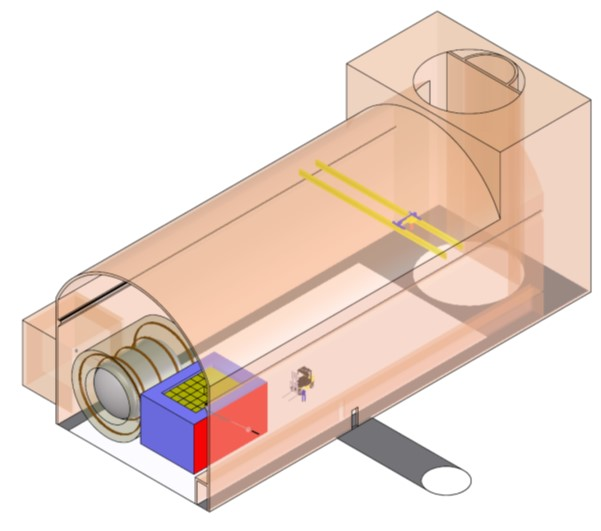
\includegraphics[width=0.49\textwidth]{graphics/NDHall_onaxis.jpg}
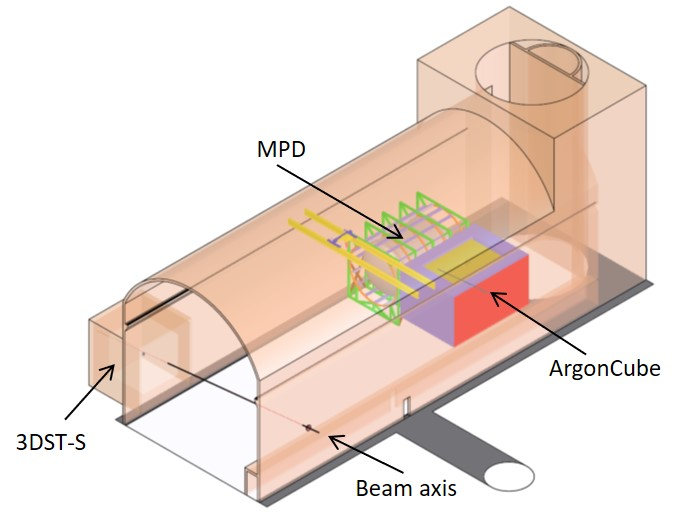
\includegraphics[width=0.49\textwidth]{graphics/NDHall_offaxis.jpg}
\end{dunefigure}

The \dword{lartpc} begins to lose acceptance for muons above a momentum of 
$\approx$0.7~GeV/c since the muons will not be contained in the \dword{lartpc} volume.  Since the muon momentum is a critical component of the neutrino energy determination, a magnetic spectrometer is needed downstream of the \dword{lartpc} to measure the charge sign and momentum of the muons.  In the \dword{dune} \dword{nd} concept, this function is accomplished by the multipurpose detector (\dword{mpd}) which consists of a \dword{hpgtpc} surrounded by an \dword{ecal} in a \SI{0.5}{T} magnetic field. The \dword{hpgtpc} provides a lower density medium with excellent tracking resolution for the muons from the \dword{lartpc}.  

In addition, neutrinos interacting on the argon in the gas \dword{tpc} constitute a sample of $\nu$-argon events that can be studied with a very low charged-particle tracking threshold and excellent resolution superior to liquid argon. The high pressure yields a sample of $\num{2e6}{\numu \text{-CC events/year}}$ for these studies. These events will be valuable for studying the charged particle activity near the interaction vertex since this detector can access lower momenta protons than the \dword{lar} detector and has better particle identification of charged pions.  The lack of secondary interactions in these samples will be helpful for identifying the particles produced in the primary interaction and modeling secondary interactions in denser detectors, which are known to be important \cite{Friedland:2018vry}.

The \dword{lartpc} and \dword{mpd} can be moved sideways up to 33~m to take data in positions off the beam axis.  This capability is referred to as \dword{duneprism}. As the detectors move off-axis, the incident neutrino flux spectrum changes, with the mean energy dropping and the spectrum becoming more monochromatic.  Though the neutrino interaction rate drops off-axis, the intensity of the beam and the size of the \dword{lartpc}  combine to yield ample statistics even in the off-axis positions.
The DUNE concept is based on reconstructing the energy-dependent neutrino spectrum and
their comparison between the far and near site. The capability of modifying the energy spectrum at the near site through measuring at the off-axis locations will allow to disentangle otherwise degenerate effects due due systematic biases om the energy reconstruction.

The final component of the \dword{dune} \dword{nd} suite is the on-axis beam monitor which contains the
\dword{3dsts} tracker within the magnet of the KLOE detector.  The \dword{3dst} is a plastic scintillator detector made of \SI{1}{cm} cubes that are read out along each of three orthogonal dimensions.  
This device importantly serves as a dedicated  neutrino spectrum monitor that stays on-axis  when the \dword{lartpc} and \dword{mpd} have moved to an off-axis position. 
It also provides an excellent on-axis neutrino flux determination that can be used as an important point of comparison and a systematic crosscheck for the flux as determined by the \dword{lartpc}.


%%%%%%%%%%%%%%%%%%%%%%%%%%%%%%%%
\section{International Organization and Responsibilities}

DUNE is the first science project of this scale in the United States that will be built with large
international participation and as an international collaboration. As such, DUNE requires a new organizational and governance model that takes into account the international nature of the project.
The
model used by CERN for managing the construction and exploitation of the Large Hadron Collider (LHC) and its experiments served as a starting point for the joint management of LBNF and the DUNE experimental program. 
LBNF, which is responsible for the facilities, comprising the neutrino beam, the near site at \fnal and the far site at \surf, is organized as a
DOE-\fnal project incorporating international partners. 
DUNE is a fully international project
organized by the DUNE collaboration with appropriate oversight from all international stakeholders.
The DUNE collaboration is responsible for
\begin{itemize}
\item the definition of the scientific goals and corresponding scientific and technical requirements on the detector systems and neutrino beamline;
\item the design, construction, commissioning, and operation of the detectors; and
\item the scientific research program conducted with the DUNE detectors. 
\end{itemize}

A set  of  organizational structures  has been established  to  provide
coordination  among  the  participating  funding agencies;
oversight of the LBNF and DUNE projects;
and coordination and communication between the 
two. These structures and the relationships among them are shown 
in Figure~\ref{fig:org}. They comprise the following committees:
\begin{itemize}
\item International Neutrino Council (INC)

The INC is composed of regional representatives, such as CERN, and representatives of funding agencies making major contributions to LBNF infrastructure and to DUNE. The INC acts as the highest-level international advisory body to the U.S. Department of Energy (DOE) and the \fnal directorate. The INC facilitates high-level global coordination across the entire enterprise (LBNF and DUNE). The INC is chaired by the DOE Office of Science associate director for high energy physics and includes the \fnal director in its membership. The council meets and provides pertinent advice to the LBNF and DUNE projects through the \fnal director as needed.
\item Resources Review Board (RRB)

The RRB is composed of representatives of all funding agencies that sponsor LBNF, DUNE, and PIP-II, and the \fnal management. The RRB provides focused monitoring and detailed oversight of the DUNE collaboration, and also monitors the progress of LBNF and PIP-II. The \fnal director,  in consultation with the international funding partners for the projects, defines the membership of the RRB. A representative from the \fnal directorate chairs the RRB and organizes regular meetings to facilitate coordination and to monitor the progress of the projects. The management teams from the DUNE collaboration and the LBNF project participate in the RRB meetings and make regular reports to the RRB on technical, managerial, financial and administrative matters, as well as reporting on the status and progress of the DUNE collaboration.

\item Long-Baseline Neutrino Committee (LBNC)

The LBNC is composed of internationally prominent scientists with relevant expertise. It provides regular external scientific peer review of DUNE, and provides regular reports to the \fnal  directorate and the RRB. The LBNC reviews the scientific, technical, and managerial decisions of the DUNE experiment. The LBNC will review the \dword{tdr} for DUNE, and will provide a recommendation to the \fnal directorate and the RRB on whether to endorse the \dword{tdr}.

%review for the two projects. The LBNC reviews the scientific, technical and managerial decisions and preparations of the neutrino program. It acts effectively as an adjunct to the \fnal Physics Advisory Committee (PAC), meeting on a more frequent basis than the PAC. 

Upon request from the Fermilab director, the LBNC may employ additional DUNE and LBNF scrutiny groups for more detailed reports and evaluations. 

\item Neutrino Cost Group (NCG)

Like the LBNC, the NCG is composed of internationally prominent scientists with relevant experience.  The NCG reviews the cost, schedule, and associated risks for the DUNE experiment, and provides regular reports to the \fnal directorate and the RRB.  The NCG will review the \dword{tdr} for DUNE and will provide a recommendation to the \fnal directorate and the RRB on whether to endorse the \dword{tdr}.


\item Experiment-Facility Interface Group (EFIG)

Close and continuous coordination between DUNE and LBNF is required to ensure the success of the combined enterprise. The EFIG  oversees the interfaces between the two projects and ensures the required coordination during the design and construction phases and the operational phase of the program. This group covers areas including interfaces between the near and far detectors and the corresponding conventional facilities; interfaces between the detector systems provided by DUNE and the technical infrastructure provided by LBNF; design of the LBNF neutrino beamline and neutrino beamline operational issues that impact both LBNF and DUNE.  

\end{itemize}

\begin{dunefigure}[Structure for oversight of the DUNE and LBNF projects.]	
{fig:org}{Top-level organization structure for oversight of the DUNE and LBNF projects.}
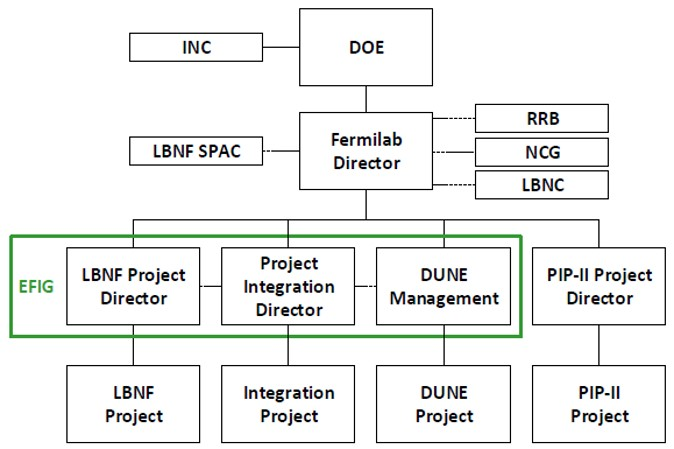
\includegraphics[width=0.67\textwidth]{graphics/lbnf_dune_org.png}  %{lbnf_dune_org.jpg} update organizational chart for consistency
%\label{fig:mhexec}
\end{dunefigure}

\section{DUNE Organization and Management}

All aspects of DUNE are organized and managed by the DUNE collaboration.  Stakeholders include the collaborating institutions, the funding agencies participating in DUNE, and \fnal as the host laboratory.  All collaborating institutions have a representative on the DUNE Institutional Board (IB). The collaboration is responsible for the design, construction, installation, commissioning, and operation of the detectors and prototypes used to pursue the scientific program. The DUNE Executive Board (EB), described below, is the main management body of the collaboration and approves all significant strategic and technical decisions.

The top-level DUNE management team consists of two elected co-spokespersons, the technical coordinator (TC), and the resource coordinator (RC). The TC and RC are selected jointly by the co-spokespersons and the \fnal director. The management team is responsible for the day-to-day management of the collaboration, and for developing the overall collaboration strategy, which is presented for approval to the executive board. The executive board consists of the leaders of the main collaboration activities. The composition of the EB, currently including the DUNE management team, IB chair, physics coordinator, beam interface coordinator, computing coordinator, near detector coordinator, and leaders of the \dword{fd} consortia, described below, is intended to ensure
that all stakeholders in the collaboration have a voice in the decision-making process (see Fig.~\ref{fig:eb}). 
In the post-TDR phase of DUNE, the intention is that the consortium leaders and the coordinators of the other major collaboration activities will become elected positions.
%, giving the full collaboration as a whole is represented in the decision-making process. 

\begin{dunefigure}[DUNE Executive Board (EB)]	
{fig:eb}{DUNE Executive Board (EB).}
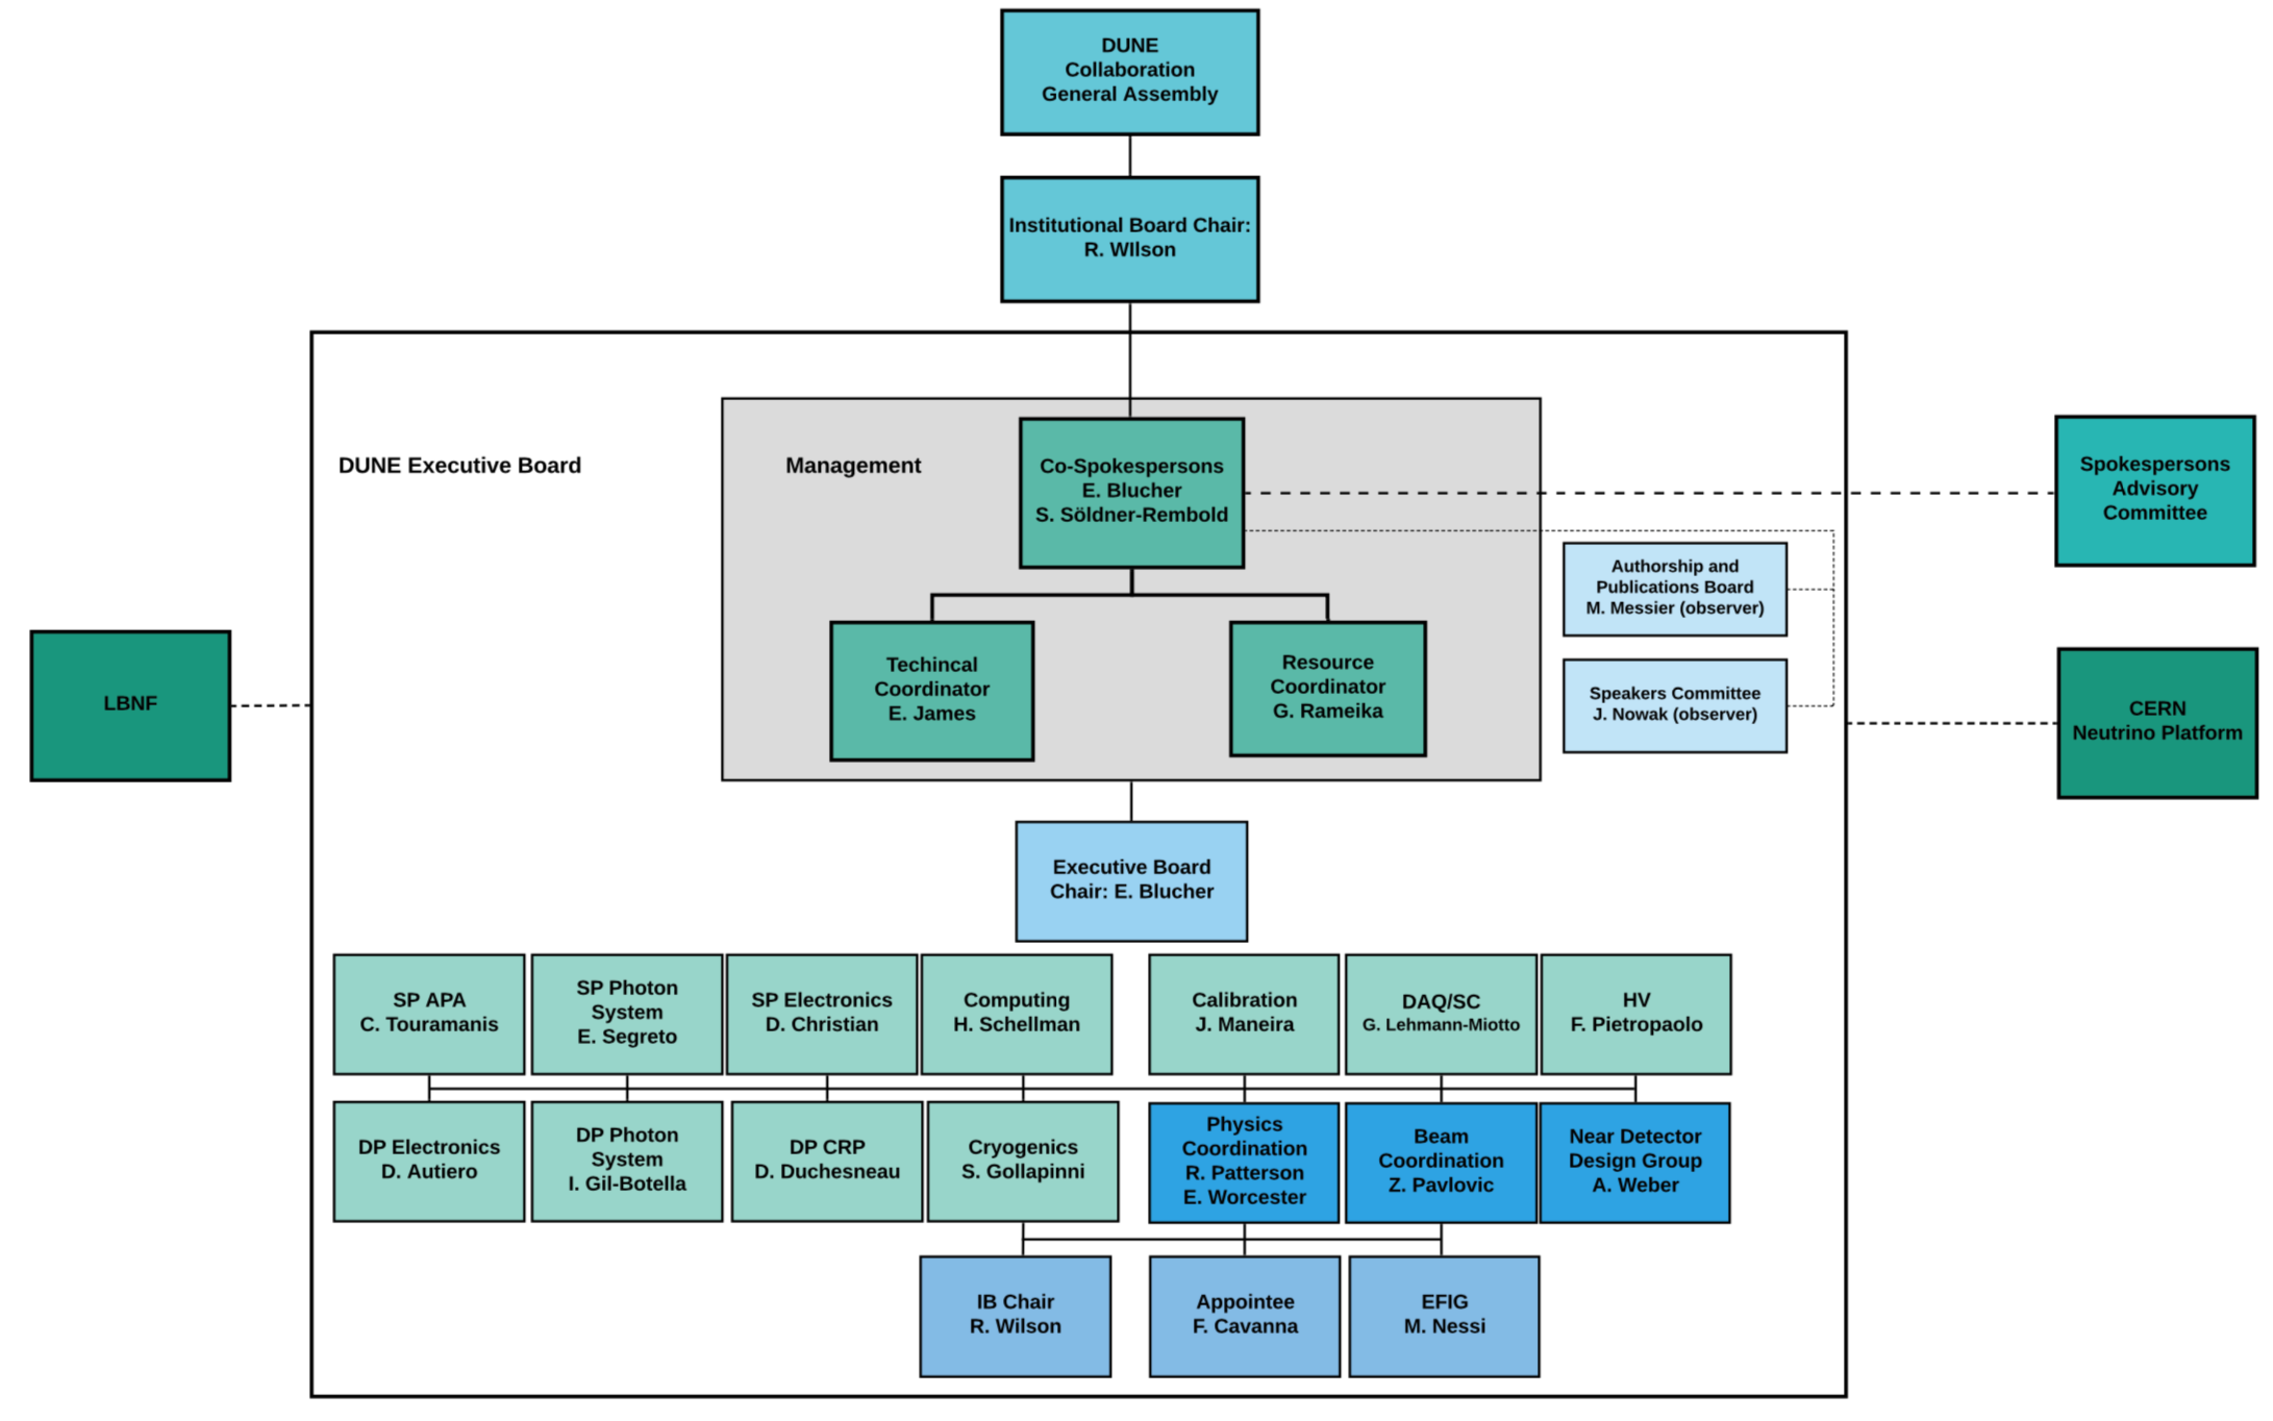
\includegraphics[width=0.9\textwidth]{graphics/eb.pdf}
\end{dunefigure}

To carry out design and construction work for the DUNE far detector, DUNE has  formed consortia of institutions that have taken responsibility for different detector subsystems. A similar structure will be formed for the DUNE near detector once the detector concept is selected. For the DUNE \dword{fd}, there are currently nine consortia, including three specific to \single, three specific to \dual, and five common to both technologies:
\begin{itemize}
\item (\single) \dwords{apa}, %Anode Plane Assemblies% (C. Touramanis, UK)
\item (\single) TPC \dword{ce}, % (D. Christian, US)
\item (\single) \dword{pds}, %Photon Detection System% (E. Segreto, Brazil)
\item (\dual) \dwords{crp}, %Charge Readout Planes% (D. Duchesneau, France)
\item (\dual) TPC electronics, %(D. Autiero, France)
\item (\dual) \dlong{pds} (PDS), %Photon Detection System %(I. Gil-Botella, Spain)
\item \dword{hv} system, %(F. Pietropaolo, CERN)
\item \dword{daq} system, %DAQ System %(D. Newbold, UK)
\item \dword{cisc} system, %Slow Controls and Instrumentation. %(S. Gollapinni, US)
\item calibration system,
\item computing.
\end{itemize} 
 Each consortium has an overall leader, a technical lead, and a consortium board with representatives from each consortium institution. The consortia have full responsibility for their subsystems, and have been responsible for development of a \dword{wbs}, understanding and documenting all interfaces with other systems, preparing final technical designs, and writing their respective sections of the \dword{tdr}. Following approval of the  \dword{tdr}, they will be responsible for construction of their detector systems. %In addition to a variety of other tasks, the consortia are responsible for writing their respective sections of the technical proposal and the TDR.


%%%%%%%%%%%%%%%%%%%%%%%%%%%%%%%%%%%%%%%%%%%%%%%%%%%%%%%%%%%%%%% new 15 May
\section{Schedule and Milestones} 

%%%%% -- added
LBNF and DUNE are working toward three international project milestones:
\begin{itemize}
\item \maincavernstartexc{}: Start main cavern excavation in South Dakota; %at \surf{}, (Anne: I added this definition)
%\item \firstfdmodstartinstall{}: Start installation of first \dword{fd} module (Anne: not defined); 
\item \startfirsttpcinstall{}: Start installation of first \dword{fd} module; 
\item \beamturnon{}: Beam operation with two \dwords{detmodule}.
\end{itemize}
It is expected that these dates will be adjusted when the project baseline is defined. 

%The key milestones to reach baseline status are:
%\begin{itemize}
%\item 2018 - Collect data with both \dword{protodune} detectors.
%\item April 2019 - Submit \dword{tdr} for far \dwords{detmodule}.
%\item July 2019 - Complete LBNC and NCG review of \dword{tdr}.
%\item September 2019 - Present \dword{tdr} to RRB.
%\item October 2019 - Conduct conceptual design (DOE CD-2/3b) review of LBNF and the USA scope of DUNE.
%\end{itemize}
%The \dword{tdr} for the near detector is expected to follow the \dword{fd} \dword{tdr} by approximately one year.

The schedule for the design and construction work for LBNF and DUNE has two critical parallel paths: one for the %Far Site scope at SURF 
far site (South Dakota) %(\surf) and %one 
another for the %Near Site scope at 
near site (Illinois). %(\fnal). 
The schedule for the initial work is driven by the \dword{cf} design and construction at each site.

During the initial phase of the project, the far site \dword{cf} is advanced first. The Ross Shaft rehabilitation
work at \surf was recently halted at the 4850 level due to safety concerns, which have led to delays of two to four months. Early site preparation is timed to be completed 
in time to start excavation when the Ross Shaft rehabilitation work finishes. As each detector 
 cavern is excavated and sufficient utilities are installed, the cryostat and cryogenics system work proceeds, followed by detector installation, filling and commissioning. 
The first \dword{detmodule} is to be operational by 2024, with the second and third modules completed one and two years later, respectively.

The DOE project management process requires approvals at critical decision (CD) milestones that allow the LBNF/DUNE project to move to the next step. In spring 2018 LBNF near site \dword{cf} will seek CD-3b construction approval for Advanced Site Preparation to build the embankment. In 2020 LBNF and DUNE will seek to baseline the LBNF/DUNE scope of work, cost and schedule, as well as construction approval for the balance of the project scope of work. 

The project concludes with CD-4 approval to start operations.


%%%%%%%%%%%%%%%%%%%%%%%%%%%%%%%%%%%%%%%%%%%%%%%%%%%%%%%%%%%%%%
\section{Organization of the DUNE Technical Design Report}

%%%%%%%%%%%%%%%%%%%%%%%%%%%%%%%%%%%
%\subsection{A Roadmap of the TDR}

The DUNE \dword{tdr} describes the proposed physics program  the experiment's proposed physics program, the 
technical designs of the two far detector \dword{lartpc} technologies, and the technical coordination required to construct and commission the first far \dwords{detmodule}.
It is intended to 
justify the technical choices that flow down from the high-level physics goals through requirements at all levels of the Project. These design choices will enable the DUNE experiment to make the ground-breaking discoveries that will help to  answer %the flagship 
fundamental physics questions. 

The DUNE far detector designs have been prototyped with the two \dword{protodune} detectors at \dword{cern}, and these designs, while largely completed, are undergoing adjustments following lessons learned. Production of detector components is being planned. 
The \dword{dune} \dword{tdr} therefore presents a final technical design for most elements and the few remaining alternative or enhanced designs that are under consideration. This \dword{tdr} represents the state of the design for the first three DUNE far detector modules.
The fourth module could employ a different \lartpc technology, taking into account  potential advances in technology, to enhance the sensitivity for physics discoveries.  The \dword{nd} \dword{tdr} is planned for 2020.

The \dword{dune} \dword{tdr} is composed of five volumes, as follows:

\begin{itemize}
\item Volume~\volnumberexec{} provides the executive summary of the overall experimental program. It includes a brief description of the DUNE science program, the DUNE detectors, and technical coordination, which are subject of the remaining volumes in the TDR. This volume also includes a description of two systems that are not yet at the technical design stage: the DUNE near detector and DUNE computing.
\item Volume~\volnumberphysics{} outlines the scientific objectives and describes the physics studies that the \dword{dune} collaboration will undertake to address them and the methods to be used.
\item Volume~\volnumbersp{} describes the \dword{sp} \dword{fd} technology, the subsystems and components that will comprise the first (and any subsequent) \dword{sp} \dwords{detmodule}, and the installation plan for the first \dword{fd} module, which will be of this type. 
\item Volume~\volnumberdp{} describes the \dword{dp} \dword{fd} technology, the subsystems and components that will comprise the first (and any subsequent) \dword{dp} \dwords{detmodule}, and the installation plan for the first \dword{dp} module. 
\item Volume~\volnumbertc{} describes the organizational structures,  methodologies, procedures, requirements, risks and other technical  coordination aspects of constructing the first two \dword{fd} modules in South Dakota.
\end{itemize}

